\paragraph{QuizziPedia::Front-End::ModelViews::ResultsOfQuizzesModelView}
	
	\label{QuizziPedia::Front-End::ModelViews::ResultsOfQuizzesModelView}
	
	\begin{figure}[ht]
		\centering
		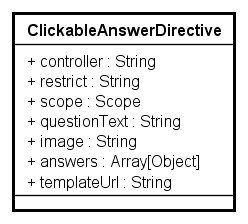
\includegraphics[scale=0.5,keepaspectratio]{UML/Classi/Front-End/QuizziPedia_Front-end_Templates_ClickableAnswerTemplate.png}
		\caption{QuizziPedia::Front-End::ModelViews::HomeModelView}
	\end{figure} \FloatBarrier
	
	\begin{itemize}
		\item \textbf{Descrizione}: classe di tipo modelview la cui istanziazione è contenuta all'interno della variabile di ambiente \$scope di \textit{Angular.js\ped{G}}. All'interno di essa sono presenti le variabili e i metodi necessari per il \textit{Two-Way Data-Binding\ped{G}} tra la view \texttt{ResultsView} e il controller \texttt{ResultsController};
		\item \textbf{Utilizzo}: viene utilizzata per effettuare il \textit{Two-Way Data-Binding\ped{G}} tra la view \texttt{ResultsView} e il controller \texttt{ResultsController} rendendo disponibili variabili e metodi;
		\item \textbf{Relazioni con altre classi}: 
		\begin{itemize}
			\item \textit{IN} \texttt{ResultsView}: view contenente i risultati della ricerca effettuata, sia gli utenti che i questionari trovati; 
			\item \textit{IN} \texttt{ResultsController}: questa classe permette di gestire le iscrizione degli utenti ai questionari;
		\end{itemize}
		\item \textbf{Attributi}: 
		\begin{itemize}
			\item \texttt{+ results: Array} \\ Array contenente un oggetto per ogni iscritto che ha compilato il questionario. L'oggetto sarà composto dai campi: \texttt{nome} e \texttt{cognome} e \texttt{valutazione}.
		\end{itemize}
	\end{itemize}
	
	